\documentclass[12pt]{article}
\usepackage[a4paper, margin=1in, headheight=14pt]{geometry}
\usepackage[utf8]{inputenc}
\usepackage[spanish]{babel}
\usepackage{hyperref}
\hypersetup{
    unicode=true, % Use non-Latin characters in Acrobat's bookmark
    pdffitwindow=false, % window fit to page when opened
    colorlinks=false, % Gives color to the links
    bookmarks=true,
    linktoc=all
}
\usepackage{tabularx}
\usepackage{graphicx}
\usepackage{float}
\usepackage[xindy, nomain, acronym, acronyms, nonumberlist, nopostdot, toc, section=section,nogroupskip]{glossaries}
\usepackage[automake]{glossaries-extra}
\usepackage{setspace}
\usepackage{anyfontsize}
\usepackage[toc,page]{appendix} % Remove toc,page to render wo appendix

\usepackage{nameref}
\usepackage{datetime}
\usepackage[table]{xcolor}
\usepackage{colortbl}
\usepackage{changepage}
\usepackage{longtable}
\usepackage{makecell}
\usepackage{multicol}
\usepackage{amssymb}
\usepackage{chngcntr} % counterwithin
\counterwithin{figure}{section}
\counterwithin{table}{section}
\usepackage{enumerate}
% New Commands
\newcommand{\nombredelproyecto}{Banco Chupi Guay (nombre provisional inspirado por los controles de FAL)}

\setcounter{secnumdepth}{4}
\makeatletter
\renewcommand{\paragraph}{\@startsection{paragraph}{4}{0ex}%
    {-3.25ex plus -1ex minus -0.2ex}%
    {1.5ex plus 0.2ex}%
    {\normalfont\normalsize\bfseries}}
\makeatother

\definecolor{riskred}{HTML}{CC4125}
\definecolor{riskyellow}{HTML}{FFD966}
\definecolor{riskgreen}{HTML}{6AA84F}
\definecolor{riskpurple}{HTML}{B4A7D6}
\definecolor{riskblue}{HTML}{00FFFF}

\title{\nombredelproyecto} 
\author{Alejandro Barrachina Argudo \\
David Cantador Piedras \\
Rodrigo Sosa Sáez \\
Juan Pantaleón Femenía Quevedo \\
David Llanes Martín \\
Sergio Sánchez Chamizo  \\
Samuel Rodríguez Moreno \\
Rodrigo Souto Santos
}

\makeglossaries
\newabbreviation{bd}{BD}{Base de Datos}
\newabbreviation{jvm}{JVM}{Máquina Virtual de Java}
\newabbreviation{sql}{SQL}{Structured Query Language}
\newabbreviation{rup}{RUP}{Rational Unified Process}
\newabbreviation{mg}{MG}{Módulo Gestor}
\newabbreviation{mc}{MC}{Módulo Cliente}
\newabbreviation{dd}{DD}{Descentralizada Democrática}
\newabbreviation{ldc}{LDC}{Lineas de Código}
\newabbreviation{pf}{PF}{Puntos de Función}
\newabbreviation{is}{IS}{Ingeniería del Software}

\newglossaryentry{host}{
	name = host,
	sort = host,
	description = {Equipo que funciona como punto de inicio y fin de las transferencias de datos para el resto de ordenadores conectados a la red, bien sea local o bien sea global.}
}

\newglossaryentry{sqa}{
	name = SQA,
	sort = sqa,
	description = {conjunto de actividades planificadas y sistemáticas, cuyo primer objetivo es evaluar la calidad y la adherencia de los productos de software a los estándares, procesos y procedimientos.}
}


\date{\today}

\begin{document}
\begin{titlepage}
	\makeatletter
	{
		\centering
		\vspace*{4cm}
		{\fontsize{40pt}{40pt}\scshape\textbf{\@title}\par}


		{\Huge Plan de proyecto\par}

		\vspace*{1cm}
		{\Large\itshape
			\@author
			\par}
	}
	\vfill
	\makeatother
\end{titlepage}
\newpage

\section*{Control de cambios} %
\noindent\begin{tabularx}{\textwidth}{ |l|l|p{5cm}|X| }
	\hline
	\textbf{Versión} & \textbf{Fecha} & \textbf{Autores}     & \textbf{Descripción}                                \\
	\hline
	0.1              & 15/12/2020     & Alejandro Barrachina & Inicio del PDP y comienzo del apartado introducción \\
	\hline
	                 &                &                      &                                                     \\
	\hline
	                 &                &                      &                                                     \\
	\hline
	                 &                &                      &                                                     \\
	\hline
	                 &                &                      &                                                     \\
	\hline
	                 &                &                      &                                                     \\
	\hline
\end{tabularx}

\newpage
\tableofcontents
\newpage
\section{Introducción}
\subsection{Propósito del plan}
\begin{itemize}
	\item Tener un texto formal con las planificaciones, estrategias y acciones estimadas para realizar el proyecto de forma ordenada y completando plazos.
	\item Tener en cuenta plazos, riesgos, actividades, equipo, costes, cambios, etc. Todo de forma ordenada para que el trabajo que se ejecute siga la dirección que necesitamos.
\end{itemize}

\subsection{Ámbito del proyecto y objetivos}
\subsubsection{Declaración del proyecto}
Esta aplicación está dirigida a bancos que quieran dar soporte online a sus clientes en sus operaciones del día a día como gestionar sus ingresos, recibir su nómina o comprar y vender acciones.
\subsubsection{Funciones principales}
El software permitirá la gestión de tareas básicas para el usuario y para el propio banco. Estas acciones incluyen la gestión de cuentas, tarjetas bancarias, prestamos, acciones y la actividad general de la cuenta.
\subsubsection{Aspectos de rendimiento}
Todas las funciones a excepción del renderizado de la interfaz están gestionadas por el servidor de la propia tienda, por lo tanto estará limitado por la potencia del servidor, las conexiones concurrentes al mismo y la potencia del ordenador del usuario y de su velocidad de red.
\subsubsection{Restricciones y técnicas de gestión}
En las funciones principales de gestión de usuarios se pedirá el DNI y la contraseña del usuario.

\noindent La baja de dicho usuario se ejecutará si y solo si el usuario ya está registrado en la \gls{bd}.

Las funciones más importantes de un usuario requerirán de su firma electrónica, para así verificar con más seguridad que no se trata de una suplantación y evitar problemas tanto al cliente como al banco.

Las funciones principales de gestión del gestor, el alta de un gestor y para la baja de un gestor al igual que las anteriores se necesita que el gestor esté registrado en la \gls{bd}.

\subsection{Modelo de proceso}
Se va a usar el modelo de proceso \gls{rup}, basado en componentes conectados a través de interfaces y dirigido por casos de uso. En espiral, de forma iterativa se siguen las siguientes fases de desarrollo:
\begin{itemize}
	\item\textbf{Requisitos (Comunicación):} mediante la comunicación con el cliente se realiza una especificación de los requisitos que deberá cumplir la aplicación.
	\item\textbf{Análisis (Planteamiento):} se crea un plan de proyecto evaluando los riesgos, se definen las características y funciones mediante casos de uso preliminares. Se crea una arquitectura basada en subsistemas o componentes muy genérica, que deberá ser desarrollada durante la fase de diseño mediante modelado.
	\item\textbf{Diseño (Modelado):} Se mejoran y amplían los casos de uso de la fase de análisis. Se modelan los subsistemas y se realiza la línea de base de la arquitectura del sistema.
	\item\textbf{Implementación (Construcción): }Se desarrollan o adquieren los componentes del software necesario para completar los casos de uso necesarios. Se completan los modelos (requisitos, casos de uso, etc.) para poder implementarlos en código fuente y se efectúan pruebas unitarias de cada uno de los componentes. También se deben realizar pruebas de integración para comprobar que la aplicación funciona.
	\item\textbf{Prueba (Despliegue):} los usuarios finales o una muestra de estos realizan pruebas Beta\footnote{Beta: fase de desarrollo de un software en la que se realiza una eliminación de errores de forma activa}, que reportan los defectos y carencias del software. En esta fase se generan también los manuales de usuario, paquetes de instalación. plataformas de ayuda necesarias para el lanzamiento.
\end{itemize}

Al finalizar la fase de despliegue tenemos una aplicación funcional que puede ser usada. Se incrementa la versión del software y se realiza la siguiente iteración del proceso. Nosotros nos encontramos en esta entrega en la fase de elaboración (que incluye parte de los requisitos, pero sobre todo análisis) de la primera iteración.

\newpage
\section{Estimaciones del proyecto}
\subsection{Datos históricos}
Este grupo no ha realizado proyectos anteriormente, y ninguno de los componentes
cuenta con experiencia en proyectos usando Ingenieríıa del Software, por lo que se carece
de datos históricos para hacer las estimaciones.
\subsection{Técnicas de estimación}
Se va a utilizar una técnica de estimación basada en la descomposición del proceso
(EDT) de este modo podremos descomponer el proyecto en funciones principales y en tareas
lo que nos dará la posibilidad de realizar una estimación del costo y del esfuerzo del proyecto
de forma escalonada.

\subsection{Estimaciones de esfuerzo, coste y duración}
La fecha de comienzo del proyecto fue el 1 de octubre de 2020 y dedicando 2 días a la semana para su desarrollo. Este proyecto no tendrá ningún coste de carácter económico, sólo tendrá un coste de esfuerzo.
La estimación de esfuerzo por cada uno de los módulos del sistema que se desarrollan en el proyecto son:
\begin{itemize}
	\item \textbf{\gls{mg}}: El programa podrá gestionar las cuentas de los clientes  y la gestión de los préstamos.Los clientes nuevos se  podrán crear una cuenta nueva,  añadir tarjetas nuevas  y aprobar o denegar préstamos. Los clientes que ya tengan cuenta, se les podrá cambiar el titular, la clave de seguridad o eliminar la cuenta, así como cambiar el pin de la tarjeta o desbloquearla y también se les podrá aprobar o denegar los préstamos. Se estima que para este módulo se necesitarán ocho iteraciones para completarlo. En este módulo intervendrán dos miembros del equipo en el análisis, tres en el diseño, dos en la codificación y dos en las pruebas.
	\item \textbf{\gls{mc}}: El programa gestiona parte de las cuentas del cliente,  las tarjetas de dicho cliente y la gestión de las acciones del cliente. Los clientes podrán actualizar datos como, sus nóminas, hacer transferencias, contactar con los gestores o solicitar un préstamo, así como  comprar y vender acciones y gestionar sus tarjetas, bloqueándolas, descargándolas o cargándolas. Se estima que para este módulo se necesitarán cinco iteraciones para completarlo. En este módulo intervendrán tres miembros del equipo en el análisis, cuatro en el diseño, tres en la codificación y tres en las pruebas.
\end{itemize}

Suponiendo que se trabajará 8 horas diarias, durante 22 días al mes sacamos los siguientes resultados cuya medida sería persona-día(pd). Un día tiene 22(pd)

\begin{table}[H]
	\begin{adjustwidth}{-1cm}{-1cm}
		\small
		\centering
		\noindent\begin{tabularx}{1.13\textwidth}{|>{\columncolor[gray]{0.8}}X|X|X|X|X|X|X|p{1.7cm}|}
			\hline
			\rowcolor{gray}
			Módulo     & Planificación & A. de Riesgo & Análisis    & Diseño      & Codificación & Prueba      & Esf. Total \\
			\hline
			\gls{mg}   &               &              & 44          & 66          & 44           & 44          & 198        \\
			\hline
			\gls{mc}   &               &              & 66          & 88          & 66           & 66          & 286        \\
			\hline
			Esf. Total & 11            & 11           & 110         & 154         & 110          & 110         & 506        \\
			\hline
			Pct        & 2,173913043   & 2,173913043  & 21,73913043 & 30,43478261 & 21,73913043  & 21,73913043 & 100\%      \\
			\hline
		\end{tabularx}
		\caption{Estimaciones del proyecto}
		\label{tab:est_proy}
	\end{adjustwidth}
\end{table}

\newpage
\section{Estrategia de gestión de riesgo}
En este apartado vamos a tratar la gestión de riesgo de un banco online, la cual consiste en tratar todos los posibles riesgos que pueden darse y cómo tratarlos de la mejor manera posible incluso antes de que sucedan,  se va a utilizar una estrategia de gestión proactiva es decir, anticiparse a los problemas o crisis que pueden suceder para minimizar los problemas.\\
Para analizar los riesgos vamos a tratar todos los casos de uso que nos han tocado.

\subsection{Introducción: Estudio de los riesgos}
A continuación vamos a indicar todos los posibles riesgos que pueden ocurrir y por cada uno de ellos, indicaremos la frecuencia con la que pueden darse, la descripción de dicho riesgo, la severidad o cuánto de grave es ese problema para el banco y sus consecuencias.
Para ello vamos a utilizar una tabla SQAS-SEI.
\begin{table}[H]
	\centering
	\small
	\begin{tabularx}{\textwidth}{|>{\columncolor[gray]{0.8}}p{3cm}|p{1.9cm}|p{3cm}|p{2.1cm}|X|}
		\hline
		\rowcolor{gray}
		Riesgo                                  & Frecuencia & Descripción                                                                     & Severidad    & Consecuencias                                                                                                                                                                                                                                     \\
		\hline
		Error al iniciar sesión                 & Frecuente  & El usuario no puede iniciar sesión                                              & Serio        & Al no poder iniciar sesión, no puede realizar ningún tipo de acción dentro del banco..                                                                                                                                                            \\
		\hline
		Error al cerrar sesión                  & Frecuente  & El usuario no puede cerrar sesión                                               & Despreciable & No es un problema grave ya que aunque no puede cerrar sesión, no afecta a nada ya que dicho cliente puede realizar todo tipo de acción dentro del banco.                                                                                          \\
		\hline
		Error al crear una cuenta al cliente    & Probable   & El gestor no puede crear una cuenta al cliente                                  & Menor        & Es similar al no iniciar sesión ya que no puede realizar ningún tipo de acción dentro del banco..                                                                                                                                                 \\
		\hline
		Error al eliminar una cuenta al cliente & Ocasional  & El gestor no puede eliminar la cuenta de un cliente                             & Menor        & Es algo más importante que no poder cerrar sesión ya que un banco se lleva un porcentaje mientras seas de ese banco, con lo que no poder eliminar tu cuenta afecta directamente al saldo del cliente el cual quiere darse de baja de dicho banco. \\
		\hline
		Error al seleccionar un cliente         & Probable   & El gestor no puede acceder a un cliente para modificar sus datos en la \gls{bd} & Serio        & Imposibilita al gestor modificar tus datos o actualizarlos con lo cual es algo serio ya que el cliente siempre quiere tener sus datos actualizados cuanto antes y no tener errores en sus cuentas.                                                \\
		\hline
	\end{tabularx}
	\caption{Tabla SQA-SEI 1}
\end{table}


\begin{table}[H]
	\centering
	\small
	\begin{tabularx}{\textwidth}{|>{\columncolor[gray]{0.8}}p{3cm}|p{1.9cm}|p{3cm}|p{2.1cm}|X|}
		\hline
		Error al cargar tarjeta del cliente         & Remoto     & El cliente no puede cargar su tarjeta de débito con el dinero que posee en su cuenta bancaria, lo cual suponemos que ha sido por un error del banco. & Crítico & Es un problema crítico casi catastrófico, estamos hablando de un dinero que le pertenece con lo que no poder acceder a su dinero afectaría muy negativamente a la confianza de la persona con el banco.                                                                                             \\
		\hline
		Error al descargar la tarjeta del cliente   & Remoto     & El cliente no puede descargar su tarjeta débito con el dinero que posee en su tarjeta                                                                & Menor   & No es algo muy grave, ya que puedes seguir utilizando el dinero que tienes en la tarjeta y no habría problemas mayores.                                                                                                                                                                             \\
		\hline
		Error al contactar con un gestor            & Remoto     & El cliente no es capaz de contactar con el gestor a través de la página de contacto diseñada para ello                                               & Menor   & Las consecuencias no son demasiado relevantes, sin embargo, puede tener un problema importante y si no contacta con un gestor puede agravarse aún más, aparte de que el cliente perderá su confianza con el banco.                                                                                  \\
		\hline
		Error al cambiar el pin de la tarjeta       & Improbable & El gestor no puede cambiar el pin de la tarjeta de un cliente                                                                                        & Menor   & No supone un problema tan grave ya que simplemente puede seguir usando la tarjeta de forma normal sin cambiar de pin ya que suponemos que conoce su pin anterior, en el caso de que lo quiera cambiar porque se haya olvidado puede preguntar al banco cuál era su pin, sin necesidad de cambiarlo. \\
		\hline
		Error al bloquear la tarjeta del cliente    & Ocasional  & El cliente no puede bloquear su tarjeta                                                                                                              & Crítico & El cliente no puede bloquear su tarjeta, y si suponemos que se la han robado es aún peor ya que este cliente no estará contento debido a que su tarjeta no pudo bloquearla y generará una gran desconfianza y una mala reputación hacia el banco.                                                   \\
		\hline
		Error al desbloquear la tarjeta del cliente & Remoto     & El cliente no puede desbloquear su tarjeta                                                                                                           & Menor   & La única consecuencia relevante es que dicho cliente no podrá usar su tarjeta, lo cual no es nada positivo y es similar al caso de no poder sacar dinero.                                                                                                                                           \\
		\hline
	\end{tabularx}
	\caption{Tabla SQA-SEI 2}
\end{table}

\begin{table}[H]
	\centering
	\small
	\begin{tabularx}{\textwidth}{|>{\columncolor[gray]{0.8}}p{3cm}|p{1.9cm}|p{3cm}|p{2.1cm}|X|}
		\hline
		Error al ingresar nómina en cuenta                                                                                                                                                   & Probable  & El cliente no puede ingresar su nómina en su cuenta personal                                                                                                                                                                                     & Crítico      & Un cliente siempre quiere tener fiabilidad con su banco, y que haya errores a la hora de ingresar la nómina es algo bastante crítico para la confianza de las personas con el banco.                                               \\
		\hline
		Error al cambiar el titular de la tarjeta                                                                                                                                            & Ocasional & El gestor no puede cambiar el titular de una cuenta                                                                                                                                                                                              & Despreciable & No afecta en nada al transcurso del dinero en sí con lo cual no es un problema grave ni prioritario.                                                                                                                               \\
		\hline
		Error al realizar una transferencia                                                                                                                                                  & Remoto    & El cliente tiene errores al intentar realizar una transferencia nacional/ internacional                                                                                                                                                          & Catastrófico & Es un problema súper grave ya que puede que haya pérdida dinero si hay fallos en las transferencias, y muchas veces las transferencias implican gran cantidad de dinero con lo que afecta a otro negocios y dificulta la economía. \\
		\hline
		Error al cambiar tu clave de seguridad                                                                                                                                               & Ocasional & El gestor no puede cambiar la clave de seguridad de la tarjeta del cliente                                                                                                                                                                       & Menor        & Al no cambiar la clave de seguridad suponemos que sí puede bloquearla con lo que, por ejemplo si se la han robado bloquea la tarjeta no podrán usarla sencillamente, por lo que no es un problema crítico                          \\
		\hline
		Error al solicitar un préstamo\newline
		---------\newline
		Error al aprobar un préstamo\newline
		---------\newline
		Error al denegar un préstamo                                                                                                                                                         & Probable  & El cliente no puede solicitar un préstamo,
		estamos suponiendo que no es problema del cliente sino fallo en el sistema de banco al no poder aprobar un préstamo, con lo cual estos tres casos de uso son prácticamente idénticos & Serio     & Muchos clientes solicitan préstamos y es algo bastante común en los bancos, que cuya principal fuente de ingresos de estos es el interés que reciben de los préstamos con lo que que haya fallos en un proceso tan importante es bastante serio.                                                                                                                                                                                                                                                     \\
		\hline
	\end{tabularx}
	\caption{Tabla SQA-SEI 3}
\end{table}

\begin{table}[H]
	\centering
	\small
	\begin{tabularx}{\textwidth}{|>{\columncolor[gray]{0.8}}p{3cm}|p{1.9cm}|p{3cm}|p{2.1cm}|X|}
		\hline
		Error al comprar acciones por parte del cliente & Improbable & El cliente no puede comprar acciones debido a un fallo en el sistema del banco & Crítico      & Comprar y vender acciones es algo súper común que mueve muchísimo dinero y prácticamente con lo que se mueven muchísimas empresas grandes, no es algo catastrófico ya que al poder comprar acciones el cliente no pierde dinero, pero tampoco lo gana, con lo que perderá mucha credibilidad en el banco en estos temas si fallan. \\
		\hline
		Error al vender acciones por parte del cliente  & Probable   & El cliente no puede vender acciones debido a un fallo en el sistema del banco  & Catastrófico & No poder vender acciones es un problema muy gordo, como he dicho antes, se mueve mucho dinero en la bolsa y al no poder vender acciones, el cliente puede perder mucho dinero por un fallo del banco, esto generaría una desconfianza brutal en todos los aspectos del banco.                                                      \\
		\hline
	\end{tabularx}
	\caption{Tabla SQA-SEI 4}
\end{table}
\newpage
\subsection{Priorización de riesgos del proyecto}
Ahora vamos a utilizar una tabla para realizar la priorización de riesgos del proyecto, la cual la rellenamos con todos los riesgos posibles según su probabilidad y su severidad.\\
Los niveles de riesgo son:
\begin{itemize}
	\item \textbf{T: Tolerable.} Si sucede, no importa.
	\item\textbf{L: Bajo.} Si sucede, los efectos son asumibles.
	\item\textbf{M: Medio.} Si sucede, afecta a los objetivos, costes o planificación. Debería controlarse.
	\item\textbf{H: Alto.} Si sucede tiene una grave trascendencia. Debería controlarse, supervisarse y tener planes de contingencia.
	\item\textbf{IN: Intolerable.} No puede obviarse su gestión bajo ningún concepto.

\end{itemize}
\begin{adjustwidth}{0cm}{-8cm}
	\begin{multicols}{2}
		\begin{table}[H]
			\fontsize{8}{9}\selectfont
			\centering
			\begin{tabularx}{0.7\textwidth}{|>{\centering}X|>{\centering}X|>{\centering}X|>{\centering}X|>{\centering}X|X|}
				\hline
				Relación de Probabilidad y Severidad & Frecuente                                         & Probable                                                                          & Ocasional                                             & Remoto                                                                       & Improbable                                \\
				\hline
				Catastrófico                         & \cellcolor{riskred}                               & \cellcolor{riskred}   E. bloquear tarjeta del cliente \newline E. vender acciones & \cellcolor{riskred}                                   & \cellcolor{riskyellow} E. realizar una transferencia                         & \cellcolor{riskgreen} E. vender acciones  \\
				\hline
				Crítico                              & \cellcolor{riskred}                               & \cellcolor{riskred}                                                               & \cellcolor{riskyellow}                                & \cellcolor{riskgreen} E. cargar tarjeta \newline	E. ingresar nómina en cuenta & \cellcolor{riskpurple}E. comprar acciones \\
				\hline
				Serio                                & \cellcolor{riskyellow}                            & \cellcolor{riskyellow} E. seleccionar cliente\newline
				E. solicitar un préstamo\newline
				E. aprobar un préstamo\newline
				E. denegar un préstamo\newline       & \cellcolor{riskgreen} E. eliminar cuenta          & \cellcolor{riskpurple}                                                            & \cellcolor{riskblue}                                                                                                                                                             \\
				\hline
				Menor                                & \cellcolor{riskgreen} E. iniciar sesión           & \cellcolor{riskgreen}E. crear cuenta                                              & \cellcolor{riskpurple}E. cambiar clave de seguridad   & \cellcolor{riskblue} E. descargar tarjeta\newline
				E. contactar con gestor\newline
				E. desbloquear tarjeta del cliente   & \cellcolor{riskblue} E. cambiar pin de la tarjeta                                                                                                                                                                                                                                                                        \\
				\hline

				Despreciable                         & \cellcolor{riskgreen} E. cerrar sesión            & \cellcolor{riskpurple} \cellcolor{riskblue}                                       & \cellcolor{riskblue} E. cambiar titular de la tarjeta & \cellcolor{riskblue}                                                         & \cellcolor{riskblue}                      \\
				\hline
			\end{tabularx}
			\caption{Tabla de Riesgos}
			\label{tab:risk}
		\end{table}
		\vfill
		\null
		\vfill

		\fbox{\begin{tabular}{ll}
				\textcolor{riskblue}{$\blacksquare$}   & Tolerable   \\
				\textcolor{riskpurple}{$\blacksquare$} & Bajo        \\
				\textcolor{riskgreen}{$\blacksquare$}  & Medio       \\
				\textcolor{riskyellow}{$\blacksquare$} & Alto        \\
				\textcolor{riskred}{$\blacksquare$}    & Intolerable \\
			\end{tabular}}
	\end{multicols}
\end{adjustwidth}

\newpage
\subsubsection{Exposición al riesgo}

Ahora ordenaremos los riesgos de mayor a menor prioridad según la exposición al riesgo

\begin{table}[H]
	\centering
	\begin{tabularx}{0.6\textwidth}{|X|X|}
		\hline
		\multicolumn{2}{|>{\hsize=\dimexpr2\hsize+2\tabcolsep+\arrayrulewidth\relax}X|}{Error al seleccionar cliente \newline
		Error al vender acciones\newline
		Error al bloquear la tarjeta del cliente}
		\\
		\hline
		Probabilidad    & Probable  \\
		\hline
		Consecuencia    & Serio     \\
		\hline
		Nivel de riesgo & (5-0.5)\% \\
		\hline
	\end{tabularx}
	\caption{Tabla de nivel de riesgo 1}
\end{table}

\begin{table}[H]
	\centering
	\begin{tabularx}{0.6\textwidth}{|X|X|}
		\hline
		\multicolumn{2}{|>{\hsize=\dimexpr2\hsize+2\tabcolsep+\arrayrulewidth\relax}X|}{Error al seleccionar cliente \newline
		Error al solicitar un préstamo \newline
		Error al aprobar un préstamo \newline
		Error al denegar un préstamo}
		\\
		\hline
		Probabilidad    & Probable  \\
		\hline
		Consecuencia    & Serio     \\
		\hline
		Nivel de riesgo & (3-0.3)\% \\
		\hline
	\end{tabularx}
	\caption{Tabla de nivel de riesgo 2}
\end{table}

\begin{table}[H]
	\centering
	\begin{tabularx}{0.6\textwidth}{|X|X|}
		\hline
		\multicolumn{2}{|>{\hsize=\dimexpr2\hsize+2\tabcolsep+\arrayrulewidth\relax}X|}{Error al iniciar sesión}
		\\
		\hline
		Probabilidad    & Frecuente \\
		\hline
		Consecuencia    & Menor     \\
		\hline
		Nivel de riesgo & $>$2\%    \\
		\hline
	\end{tabularx}
	\caption{Tabla de nivel de riesgo 3}
\end{table}

\begin{table}[H]
	\centering
	\begin{tabularx}{0.6\textwidth}{|X|X|}
		\hline
		\multicolumn{2}{|>{\hsize=\dimexpr2\hsize+2\tabcolsep+\arrayrulewidth\relax}X|}{Error al crear cuenta}
		\\
		\hline
		Probabilidad    & Probable  \\
		\hline
		Consecuencia    & Menor     \\
		\hline
		Nivel de riesgo & (2-0.2)\% \\
		\hline
	\end{tabularx}
	\caption{Tabla de nivel de riesgo 4}
\end{table}

\begin{table}[H]
	\centering
	\begin{tabularx}{0.6\textwidth}{|X|X|}
		\hline
		\multicolumn{2}{|>{\hsize=\dimexpr2\hsize+2\tabcolsep+\arrayrulewidth\relax}X|}{Error al cerrar sesión}
		\\
		\hline
		Probabilidad    & Frecuente    \\
		\hline
		Consecuencia    & Despreciable \\
		\hline
		Nivel de riesgo & $>$1\%       \\
		\hline
	\end{tabularx}
	\caption{Tabla de nivel de riesgo 5}
\end{table}


\begin{table}[H]
	\centering
	\begin{tabularx}{0.6\textwidth}{|X|X|}
		\hline
		\multicolumn{2}{|>{\hsize=\dimexpr2\hsize+2\tabcolsep+\arrayrulewidth\relax}X|}{Error al eliminar cuenta}
		\\
		\hline
		Probabilidad    & Ocasional    \\
		\hline
		Consecuencia    & Serio        \\
		\hline
		Nivel de riesgo & (0.3-0.03)\% \\
		\hline
	\end{tabularx}
	\caption{Tabla de nivel de riesgo 6}
\end{table}

\begin{table}[H]
	\centering
	\begin{tabularx}{0.6\textwidth}{|X|X|}
		\hline
		\multicolumn{2}{|>{\hsize=\dimexpr2\hsize+2\tabcolsep+\arrayrulewidth\relax}X|}{Error al cambiar clave de seguridad}
		\\
		\hline
		Probabilidad    & Ocasional    \\
		\hline
		Consecuencia    & Menor        \\
		\hline
		Nivel de riesgo & (0.2-0.02)\% \\
		\hline
	\end{tabularx}
	\caption{Tabla de nivel de riesgo 7}
\end{table}

\begin{table}[H]
	\centering
	\begin{tabularx}{0.6\textwidth}{|X|X|}
		\hline
		\multicolumn{2}{|>{\hsize=\dimexpr2\hsize+2\tabcolsep+\arrayrulewidth\relax}X|}{Error al cambiar titular de la tarjeta}
		\\
		\hline
		Probabilidad    & Ocasional    \\
		\hline
		Consecuencia    & Despreciable \\
		\hline
		Nivel de riesgo & (0.1-0.01)\% \\
		\hline
	\end{tabularx}
	\caption{Tabla de nivel de riesgo 8}
\end{table}

\begin{table}[H]
	\centering
	\begin{tabularx}{0.6\textwidth}{|X|X|}
		\hline
		\multicolumn{2}{|>{\hsize=\dimexpr2\hsize+2\tabcolsep+\arrayrulewidth\relax}X|}{Error al realizar una transferencia}
		\\
		\hline
		Probabilidad    & Remoto          \\
		\hline
		Consecuencia    & Serio           \\
		\hline
		Nivel de riesgo & (0.03-0.0003)\% \\
		\hline
	\end{tabularx}
	\caption{Tabla de nivel de riesgo 9}
\end{table}

\begin{table}[H]
	\centering
	\begin{tabularx}{0.6\textwidth}{|X|X|}
		\hline
		\multicolumn{2}{|>{\hsize=\dimexpr2\hsize+2\tabcolsep+\arrayrulewidth\relax}X|}{Error al descargar tarjeta \newline
		Error al contactar con gestor \newline
		Error al desbloquear tarjeta del cliente}
		\\
		\hline
		Probabilidad    & Remoto          \\
		\hline
		Consecuencia    & Menor           \\
		\hline
		Nivel de riesgo & (0.02-0.0002)\% \\
		\hline
	\end{tabularx}
	\caption{Tabla de nivel de riesgo 10}
\end{table}

\begin{table}[H]
	\centering
	\begin{tabularx}{0.6\textwidth}{|X|X|}
		\hline
		\multicolumn{2}{|>{\hsize=\dimexpr2\hsize+2\tabcolsep+\arrayrulewidth\relax}X|}{Error al cargar tarjeta \newline
		Error al ingresar nómina en cuenta}
		\\
		\hline
		Probabilidad    & Remoto          \\
		\hline
		Consecuencia    & Crítico         \\
		\hline
		Nivel de riesgo & (0.04-0.0004)\% \\
		\hline
	\end{tabularx}
	\caption{Tabla de nivel de riesgo 11}
\end{table}

\begin{table}[H]
	\centering
	\begin{tabularx}{0.6\textwidth}{|X|X|}
		\hline
		\multicolumn{2}{|>{\hsize=\dimexpr2\hsize+2\tabcolsep+\arrayrulewidth\relax}X|}{Error al cambiar pin de la tarjeta}
		\\
		\hline
		Probabilidad    & Improbable          \\
		\hline
		Consecuencia    & Menor               \\
		\hline
		Nivel de riesgo & (0.0002-0.000002)\% \\
		\hline
	\end{tabularx}
	\caption{Tabla de nivel de riesgo 12}
\end{table}

\begin{table}[H]
	\centering
	\begin{tabularx}{0.6\textwidth}{|X|X|}
		\hline
		\multicolumn{2}{|>{\hsize=\dimexpr2\hsize+2\tabcolsep+\arrayrulewidth\relax}X|}{Error al comprar acciones}
		\\
		\hline
		Probabilidad    & Improbable         \\
		\hline
		Consecuencia    & Crítico            \\
		\hline
		Nivel de riesgo & (0.0004-0.00004)\% \\
		\hline
	\end{tabularx}
	\caption{Tabla de nivel de riesgo 13}
\end{table}


A partir del listado anterior de los riesgos se decide qué riesgos se van a tratar, que serán
aquellos que tengan una mayor exposición. El resto de riesgos son asumidos dado la baja
probabilidad de que ocurran.

\subsection{Plan de gestión de riesgo: Reducción, supervisión y gestión de riesgo}
A continuación vamos a realizar el plan de gestión de los 2 casos de más exposición del anterior apartado (el resto de los casos son similares en muchos de los puntos), que consiste en tratar 3 puntos para cada uno, la reducción del riesgo en para que no suceda, la supervisión del mismo para comprobar si ha sucedido o no y su plan de contingencia en caso de que dicho riesgo se haya producido.\\
Como he dicho antes todos los casos se pueden resolver de una manera similar con lo que vamos a exponer los dos ejemplos de mayor exposición al riesgo.
\subsection{Riesgo 1: error al vender acciones}
\textbf{Reducción\_1:} La manera de reducir los riesgos está directamente implicada con el sistema informático ya que estamos tratando con un banco online, con lo cual toda la posible reducción de riesgos solo es posible en el terreno de la programación, esto se podría aplicar al resto de los casos también, se podría resolver mejorando todo el ámbito informático, contratando a muy buenos programadores y buenos equipos de trabajo.\\
También con el objetivo de que el problema no sea agrave mucho, solucionar los pequeños errores y darles importancia para que no se produzca un caos total, en este caso si vemos que sólo una persona de cien ha tenido problemas al vender acciones, aunque sea una persona, es probable que más personas se pueden ver afectadas más tarde, con lo que lo lógico sería solucionar dicho problema por pequeño que sea cuanto antes.

\textbf{Supervisión\_1:} Para saber si este riesgo ha sucedido podríamos saberlo de varias formas, que el ordenador detecte que hay ciertos errores al intentar vender acciones o que sea la propia persona la que pueda hacer un reporte del error, en definitiva se debería mejorar la infraestructura de la empresa para que haya métodos más efectivos a la hora de detectar errores y poder resolverlos con mucha más eficacia, y aunque no haya habido errores revisar todo el código para poder prever errores futuros.

\textbf{Plan de contingencia\_1:} Una vez ha tenido lugar este error, una de las cosas más efectivas que podríamos hacer sería tener una copia de seguridad de todo, pongámonos en el caso de que al vender acciones no recibe el dinero de dichas acciones debido a un error, con lo que al cliente le saldría que ha vendido esas acciones pero no ha recibido nada a cambio, se puede solucionar mediante una copia de seguridad en todo momento, ya que el objetivo principal es que el cliente no se vea afectado y en segundo lugar se hace una copia para volver al estado anterior del cliente para que nadie más de la empresa se vea afectado tampoco.


\subsubsection{Riesgo 2: error al bloquear la tarjeta del cliente}
\textbf{Reducción\_2:} Al igual que en el caso anterior, la gestión de la reducción de un riesgo se podría subsanar mediante una buena infraestructura informática y de esta manera evitar problemas de programación lo cual se puede resolver empleando gran cantidad de dinero a su soporte, tanto un buen mantenimiento del sistema y por supuesto un gran trato a los trabajadores (lo cual es imprescindible en una empresa) para que se sientan cómodos y puedan realizar su trabajo con mayor comodidad y eficacia.

\textbf{Supervisión\_2:} A la hora de supervisar el correcto funcionamiento de esta función, se deberá tener un buen plan de supervisión, como por ejemplo, una rápida respuesta del servidor y un buen sistema de detección de fallos con lo que es fácil saber si algo falla rápidamente ya que el ordenador nos indica si ha habido un problema que no se ha podido resolver o si hay errores e irregularidades en las cuentas de los clientes(en este caso, por ejemplo, mucho gasto de dinero porque les han robado la tarjeta y se están gastando el dinero de nuestro cliente) y también serán ellos mismos los que nos informen de ciertos problemas ya que les afecta directamente.\\
Lógicamente cada función del banco deberá ser supervisada de manera frecuente por los programadores aunque no hayan dado fallos para ver si es posible arreglar un problema que aún no ha ocurrido.

\textbf{Plan de contingencia\_3:} En el caso de que este error de a lugar, lo primero que se deberá conseguir es resolver el problema cuanto antes y de una manera rápida, mientras tanto, pongámonos en el caso de que a este cliente le han robado la tarjeta y se están gastando su dinero, pues mientras se intenta solucionar el problema, hay métodos en los bancos en los cuales no puedes sacar una gran cantidad de dinero de golpe y si ése es el caso, se consulta con el dueño de la tarjeta para ver si está de acuerdo, con lo que aunque le roben,  el gasto al menos será mínimo, y por supuesto todo gasto perdido aunque sea pequeño, lo subsanará el banco ya que el error es del mismo y a un cliente hay que garantizarle confianza y estabilidad.
Con estos pasos, se reducirá al mínimo el problema, y una vez esté solucionado mejorar dicha función y supervisarla para que no vuelva a ocurrir.

\newpage
\section{Planificación temporal}
\subsection{Estructura de descomposición del trabajo/Planificación temporal}
\begin{table}[H]
	\tiny
	\centering
	\begin{adjustwidth}{-1cm}{-1cm}
		\begin{tabularx}{1.1\textwidth}{|>{\columncolor[gray]{0.8}}p{3cm}|p{2cm}|X|X|X|X|X X|}
			\hline
			\rowcolor{gray}
			AE                                                   & Planificación y gestión de riesgo                                                               & \multicolumn{2}{|>{\hsize=\dimexpr2\hsize+2\tabcolsep+\arrayrulewidth\relax}X|}{Ingeniería} & \multicolumn{2}{|>{\hsize=\dimexpr2\hsize+2\tabcolsep+\arrayrulewidth\relax}X|}{Construcción y adaptación} & \multicolumn{2}{|>{\hsize=\dimexpr2\hsize+2\tabcolsep+\arrayrulewidth\relax}X|}{Evaluación con el cliente}                                                          \\
			\hline
			Acción                                               &                                                                                                 & Análisis                                                                                    & Diseño                                                                                                     & Codificación                                                                                               & Prueba & \multicolumn{1}{X|}{Instalación} & Evaluación \\
			\hline
			Proyecto                                             &                                                                                                 & 1.1\newline
			i: 1/10/2020 \newline
			f: 21/10/2020\newline
			r: todos\newline
			e: Análisis del proyecto                             & 1.3\newline  i: 1/10/2020\newline f: 16/10/2020\newline	r: todos \newline e: Diseño del proyecto &                                                                                             &                                                                                                            &                                                                                                            &                                                        \\
			\cline{3-3}
			                                                     &                                                                                                 & 1.2\newline
			i: 1/10/2020\newline
			f: 31/10/2020\newline
			r: todos\newline
			e: Análisis de requisitos y de funcionalidad\newline
			                                                     &                                                                                                 &                                                                                             &                                                                                                            &                                                                                                            &                                                        \\
			\hline
			Especificación de requisitos software                &                                                                                                 &                                                                                             & 2.1 \newline
			i: 1/10/2020\newline
			f: 21/10/2020\newline
			r: todos\newline
			e: Diseño de la especificación de requisitos\newline &                                                                                                 &                                                                                             &                                                                                                            &                                                                                                                                                                     \\
			\hline
			Módulo de gestión de usuarios                        &                                                                                                 & 3.1\newline
			i: 16/10/2020\newline
			f:  21/10/2020\newline
			r: A. Barrachina, D. Llanes\newline
			e: Análisis de gestión de usuarios                   & 3.2\newline
			i: 19/10/2020\newline
			f:  25/10/2020\newline
			r: A. Barrachina, D. Llanes\newline
			e: Diseño de la gestión de usuarios\newline          & 3.4\newline
			i: 1/11/2021\newline
			f:  17/11/2021\newline
			r: A. Barrachina, D. Llanes , R. Sosa\newline
			e: Codificación de la gestión de usuarios            & 3.5 \newline
			i: 17/11/2021\newline
			f:  21/11/2021\newline
			r: A. Barrachina, D. Llanes , R. Sosa\newline
			e: Prueba de la gestión de usuarios\newline          &                                                                                                 &                                                                                                                                                                                                                                                                                                                                                                                \\
			\cline{4-4}
			                                                     &                                                                                                 &                                                                                             & 3.3\newline
			i: 24/10/2020\newline
			f:  31/10/2020\newline
			r: R. Sosa, D. Llanes\newline
			e: Análisis de gestión de usuarios\newline           &                                                                                                 &                                                                                             &                                                                                                            &                                                                                                                                                                     \\
			\hline
			Módulo de gestión de servicios                       &                                                                                                 & 4.1\newline
			i: 21/11/2020\newline
			f:  31/11/2020\newline
			r: A. Barrachina, D. Cantador , R. Sosa, J. Pantaleón, S. Sánchez\newline
			e: Análisis de gestión de servicios\newline          & 4.2 \newline
			i: 16/11/2020\newline
			f:  19/11/2020\newline
			r: R. Souto, D. Cantador, S. Sánchez\newline
			e: Diseño de gestión de servicios\newline            & 4.4 \newline
			i: 19/01/2021\newline
			f:  30/01/2021\newline
			r: D. Cantador, J. Pantaleón, R. Sosa\newline
			e: Codificación de la gestión de servicios\newline   & 4.5\newline
			i: 16/01/2021\newline
			f:  19/01/2021\newline
			r: R. Souto, J. Pantaleón, S. Sánchez\newline
			e: Prueba de la gestión de servicios                 &                                                                                                 &                                                                                                                                                                                                                                                                                                                                                                                \\
			\cline{4-4}
			                                                     &                                                                                                 &                                                                                             & 4.3 \newline
			i: 21/11/2020\newline
			f:  31/10/2020\newline
			r: S. Rodríguez, R. Sosa, J. Pantaleón, S. Sánchez\newline
			e: Diseño de gestión de servicios\newline            &                                                                                                 &                                                                                             &                                                                                                            &                                                                                                                                                                     \\
			\hline
		\end{tabularx}
	\end{adjustwidth}
	\caption{Tabla de planificación 1}
\end{table}
\begin{table}[H]
	\tiny
	\centering
	\begin{adjustwidth}{-1cm}{-1cm}
		\begin{tabularx}{1.1\textwidth}{|>{\columncolor[gray]{0.8}}p{3cm}|p{2cm}|X|X|X|X|X|X|}
			\hline
			Módulo de utilidades                                      &              & 5.1 \newline
			i: 20/11/2020\newline
			f:  20/11/2020\newline
			r: A. Barrachina, D. Llanes, R. Sosa, J. Pantaleón, S. Sánchez\newline
			e: Análisis de utilidades\newline                         & 5.2\newline
			i: 21/11/2020\newline
			f:  31/11/2020\newline
			r: A. Barrachina, D. Llanes, R. Souto, J. Pantaleón, S. Rodríguez\newline
			e: Diseño de utilidades\newline                           & 5.3\newline
			i: 15/03/2021\newline
			f:  31/03/2021\newline
			r: A. Barrachina, S. Rodríguez, R. Sosa, J. Pantaleón, S. Sánchez\newline
			e: Codificación de utilidades                             & 5.4\newline
			i: 05/03/2021\newline
			f:  05/04/2021\newline
			r: A. Barrachina, S. Rodríguez, R. Souto, J. Pantaleón, S. Sánchez\newline
			e: Prueba de utilidades                                   &              &                                                                                             \\
			\hline
			Proyecto                                                  & 6.3\newline
			i: 25/11/2020\newline
			f:  02/12/2020\newline
			r: A. Barrachina, D. Cantador, R. Sosa, J. Pantaleón, S. Rodríguez\newline
			e: Revisión plan de proyecto y plan de gestión de riesgos & 6.7 \newline
			i: 21/12/2020\newline
			f:  21/12/2020\newline
			r: S. Sánchez, S. Rodríguez, R. Sosa, J. Pantaleón, S. Rodríguez\newline
			e: Cierre ingeniería                                      & 6.1 \newline
			i: 04/11/2020\newline
			f: 04/11/2020\newline
			r: R. Sosa, R. Souto, S. Rodríguez, S. Sánchez\newline
			e: Diseño final del proyecto (SRS)                        & 6.9 \newline
			i: 31/05/2021\newline
			f:  31/05/2021\newline
			r: J. Femenia\newline
			e: Entrega del código                                     &              & \multicolumn{2}{>{\hsize=\dimexpr2\hsize+2\tabcolsep+\arrayrulewidth\relax}X|}{6.2 \newline
				i: 20/05/2021\newline
				f: 20/05/2021\newline
				r: A. Barrachina, D. Cantador, R. Sosa, J. Pantaleón, S. Rodríguez\newline
				e: Corrección, estilo y entrega
			del proyecto (PDP)}                                                                                                                                                    \\
			\hline
		\end{tabularx}
	\end{adjustwidth}
	\caption{Tabla de planificación 2}
\end{table}

\newpage
\begin{landscape}
	\subsection{Diagrama de Gantt}
	\begin{figure}[H]
		\centering
		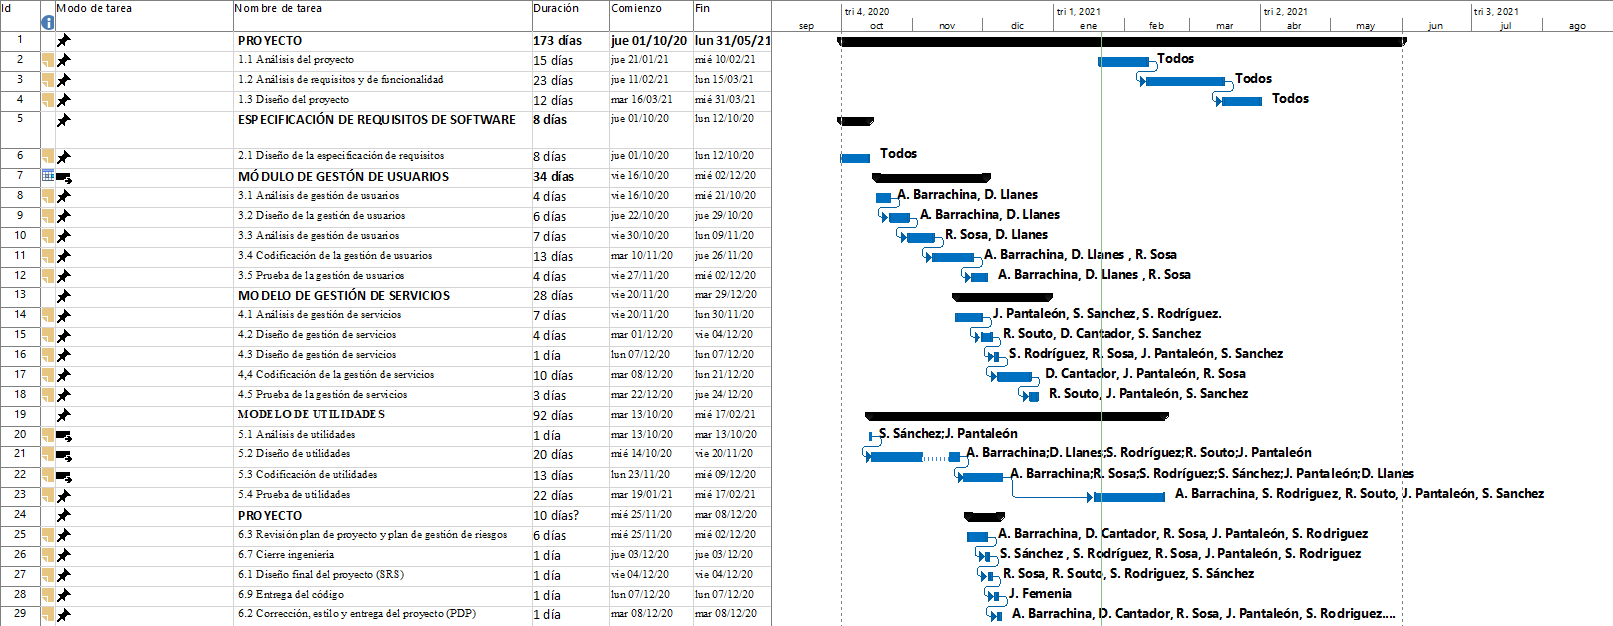
\includegraphics[width = 1.5\textwidth]{images/gantt.png}
		\caption{Diagrama de Gantt}
		\label{fig:gantt}
	\end{figure}
	\begin{figure}[H]
		\centering
		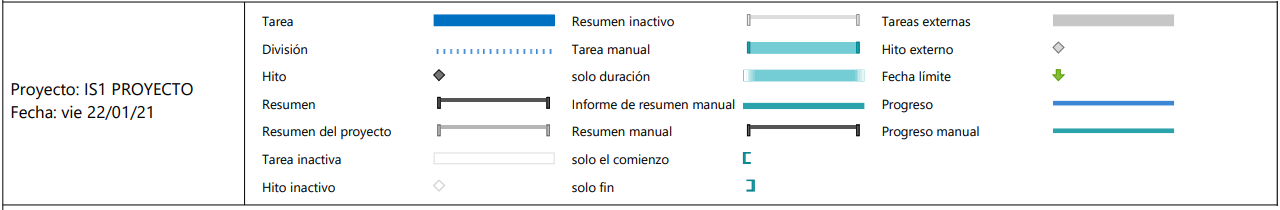
\includegraphics[width = \textwidth]{images/gantt_leyenda.PNG}
		\caption{Leyenda del diagrama \ref{fig:gantt}}
	\end{figure}
	\subsection{Red de tareas}
	\begin{figure}[H]
		\centering
		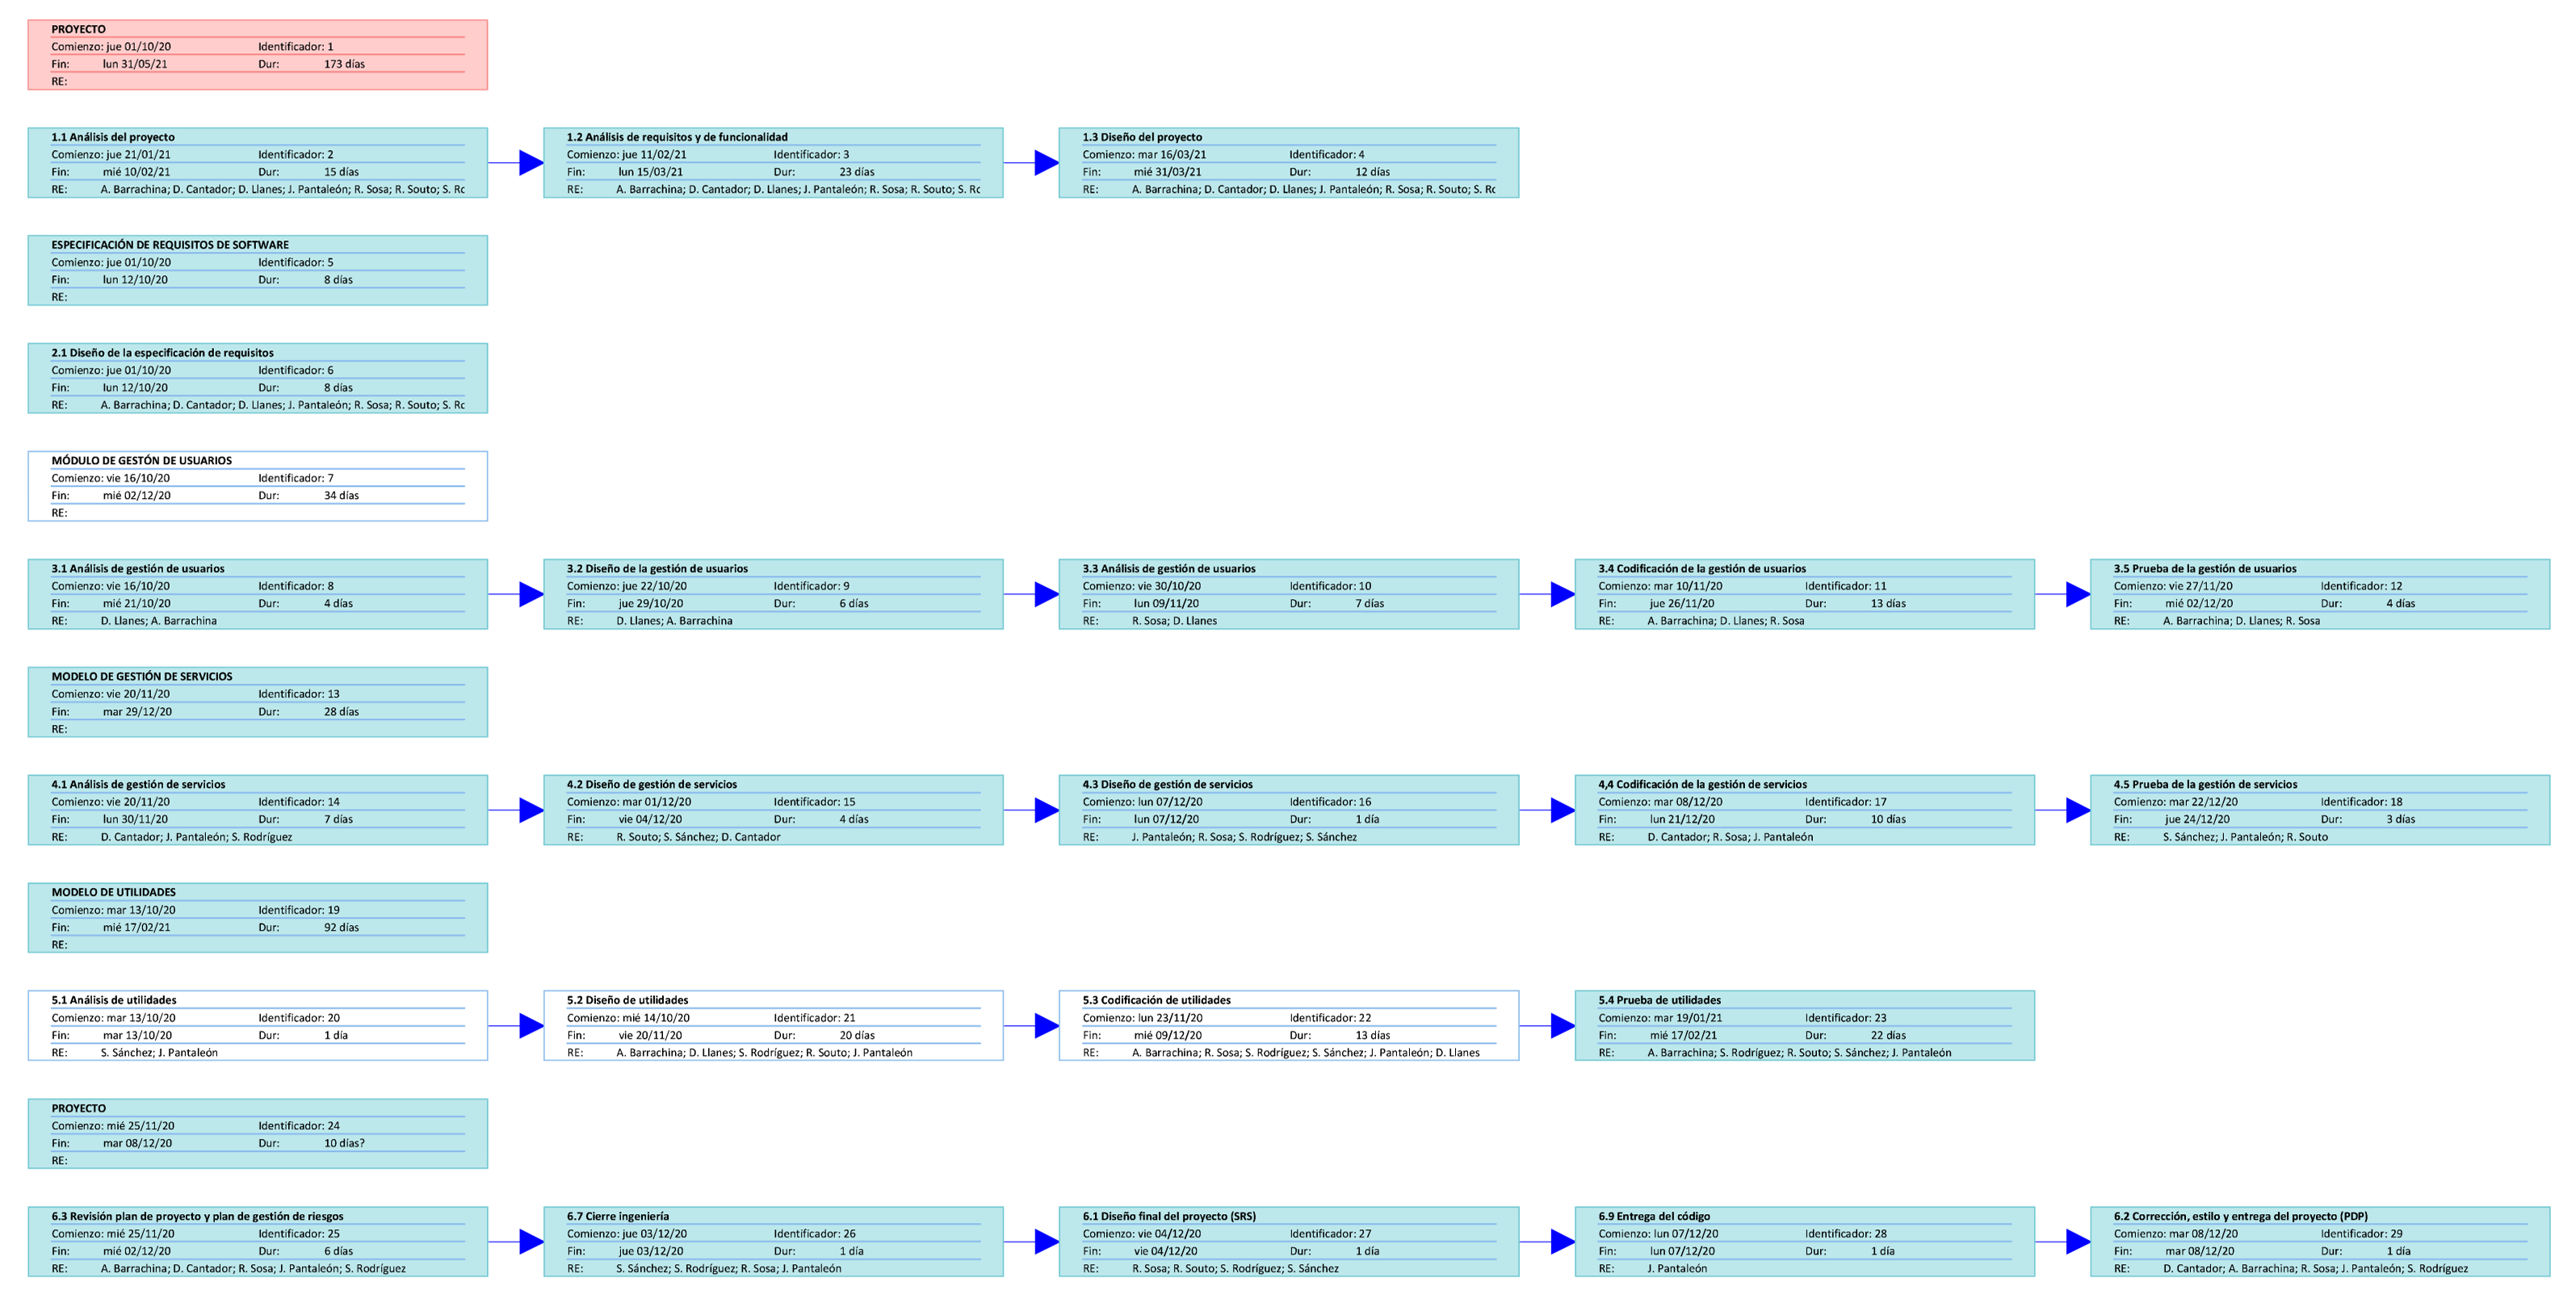
\includegraphics[width=1.5\textwidth]{images/Diagrama_Red.png}
		\caption{Diagrama en red de tareas}
	\end{figure}
\end{landscape}


\subsection{Tabla de uso de recursos}
\begin{figure}[H]
	\centering
	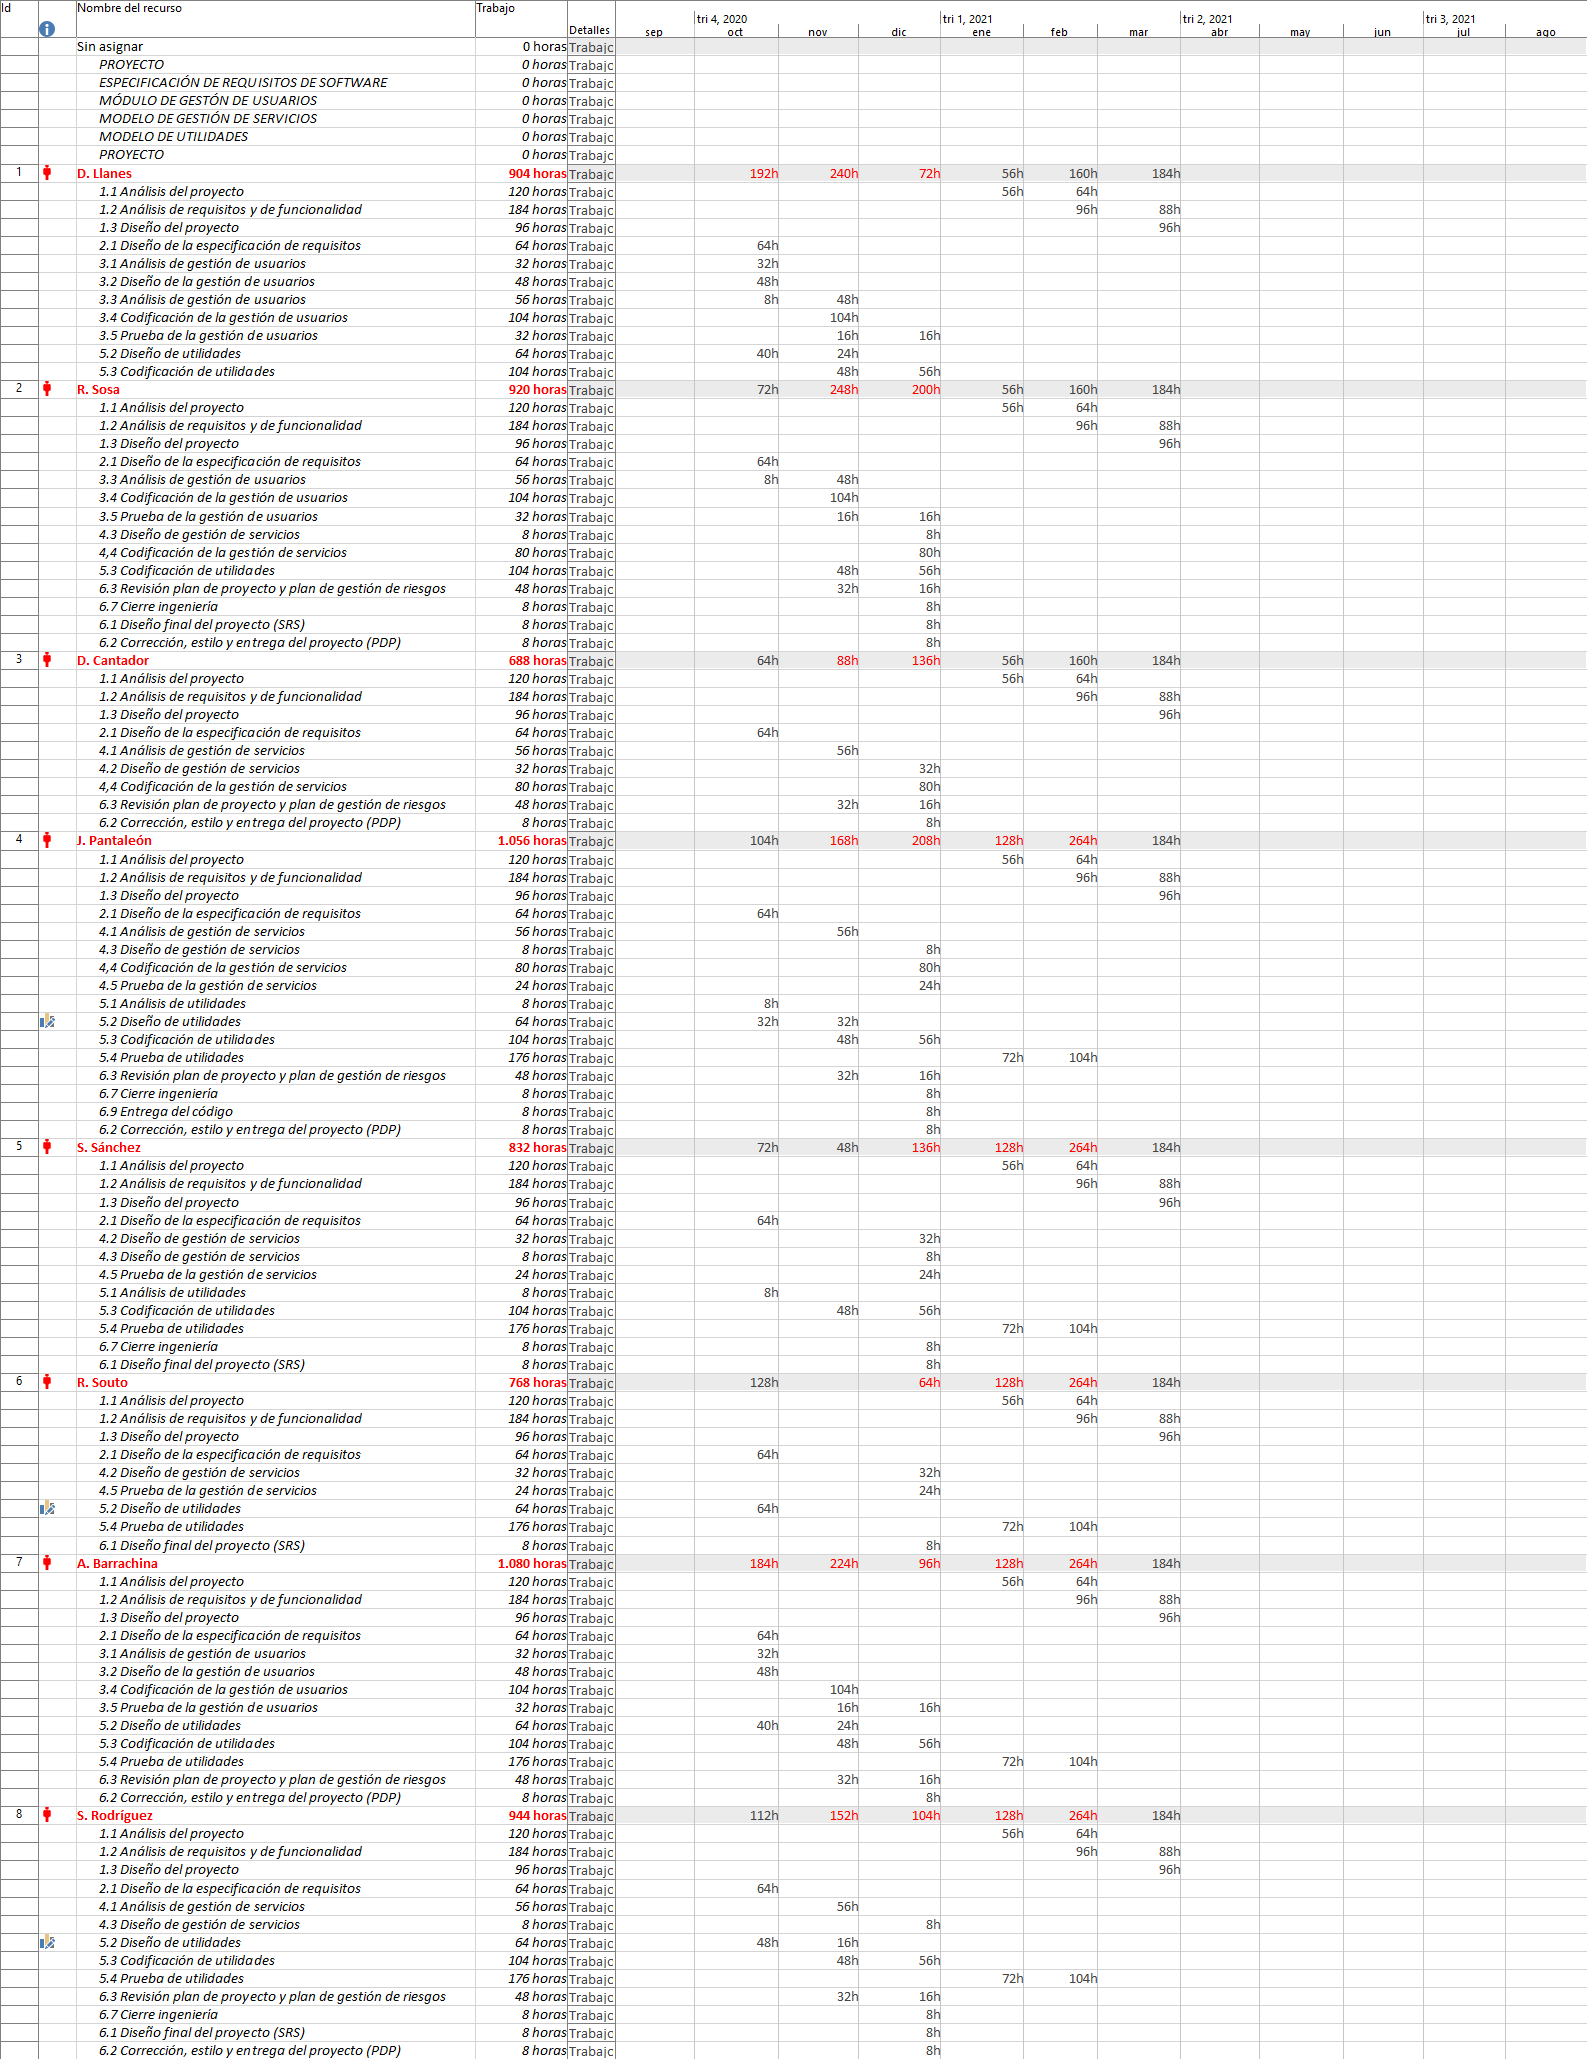
\includegraphics[width=\textwidth]{images/recursos.png}
	\caption{Uso de recursos}
\end{figure}

\newpage
\section{Recursos del proyecto}

\subsection{Personal}
\begin{itemize}
	\item \textbf{\underline{Gestor superior y Gestor técnico del proyecto}}
	      \begin{itemize}
		      \item David cantador piedras
	      \end{itemize}
	\item \textbf{\underline{Profesionales}}
	      \begin{itemize}
		      \item Alejandro Barrachina Argudo
		      \item Juan Pantaleón Femenía Quevedo
		      \item David Llanes Martín
		      \item Samuel Rodríguez Moreno
		      \item Sergio Sánchez Chamizo
		      \item Rodrigo Sosa Sáez
		      \item Rodrigo Souto Santos
	      \end{itemize}
\end{itemize}

\subsection{Hardware y software}
\begin{itemize}
	\item \textbf{\underline{Software}}
	      \begin{itemize}
		      \item \href{https://discord.com}{Discord}
		      \item \href{https://www.eclipse.org/}{Eclipse IDE for Java Developers}
		      \item \href{https://github.com}{GitHub}
		      \item \href{https://drive.google.com}{Google Drive}
		      \item \href{https://meet.google.com}{Google Meet}/ \href{https://zoom.us}{Zoom}
		      \item \href{https://www.ibm.com/products/rational-software-architect-designer}{IBM Rational Software Architect}
		      \item \href{https://www.microsoft.com/es-es/microsoft-365}{Microsoft Office}
		      \item \href{https://overleaf.com}{Overleaf}
		      \item \href{https://www.microsoft.com/es-es/microsoft-365/project/project-management-software}{Microsoft Project}
		      \item \href{https://www.oracle.com/es/enterprise-manager/technologies/}{MySQL/Oracle DBMS}
		      \item \href{https://www.microsoft.com/es-es/windows-server}{Windows Server}
	      \end{itemize}
	\item \textbf{\underline{Hardware}}
	      \begin{itemize}
		      \item Servidores rack
		      \item Puestos de trabajo
		      \item Impresoras
		      \item Fax y scanner
	      \end{itemize}
\end{itemize}

\subsection{Lista de recursos}

\begin{itemize}
	\item \textbf{\underline{Comunicación}}
	      \begin{itemize}
		      \item \textbf{Google meet/Zoom:} medio empleado para la comunicación con el stakeholder.
		      \item\textbf{Discord:} Medio empleado para la comunicación entre el personal del proyecto.
	      \end{itemize}
	\item \textbf{\underline{Entornos de almacenamiento y repositorio}}
	      \begin{itemize}
		      \item\textbf{GitHub:} medio empleado como repositorio, control de versiones y gestor de la configuración del proyecto.
		      \item\textbf{Google Drive:} medio empleado para el almacenamiento online de documentos relacionados con el proyecto.
	      \end{itemize}
	\item \textbf{\underline{Edición de documentos:}}
	      \begin{itemize}
		      \item\textbf{Microsoft Office:} paquete de programas empleado para la creación y edición de documentos  (uso mayoritario de Word)
		      \item\textbf{Overleaf:} editor online para la maquetación y edición de documentos en \LaTeX
	      \end{itemize}
	\item \textbf{\underline{Entornos de desarrollo:}}
	      \begin{itemize}
		      \item\textbf{MySQL/Oracle DBMS:} Entorno de desarrollo y gestión de la \gls{bd} asociada al producto.
		      \item\textbf{Eclipse IDE for Java Developers:} entorno de desarrollo principal para la creación del producto en lenguaje java.
		      \item\textbf{Windows Server:} entorno de gestión y control de servidores.
	      \end{itemize}
	\item \textbf{\underline{Entorno de planificación de proyectos}}
	      \begin{itemize}
		      \item\textbf{Microsoft Project:} entorno empleado para establecer la gestión del proyecto.
	      \end{itemize}
	\item \textbf{\underline{Entorno de diseño}}
	      \begin{itemize}
		      \item\textbf{IBM Rational Software Architect:} entorno empleado para diseñar la interfaz del producto.
	      \end{itemize}
	\item \textbf{\underline{Hardware}}
	      \begin{itemize}
		      \item\textbf{Servidores Rack:} Permiten que los clientes puedan acceder al servidor en cualquier momento, almacenar la \gls{bd} y hacer copias de seguridad.
	      \end{itemize}
\end{itemize}

\newpage
\section{Organización del personal (Gestión del equipo)}
\subsection{Estructura del equipo}
La organización del equipo se basa en una estructura \gls{dd}, la cual ha sido elegida por los integrantes del grupo fundamentándonos en las estructuras de equipo de Mantei.
Para ello nos hemos basado en siete factores para determinar la estructura a elegir: dificultad del problema, tamaño en \gls{ldc} o \gls{pf}, duración del equipo, modularidad del problema, calidad y fiabilidad, fecha de entrega, comunicación requerida en el proyecto.

\begin{figure}[H]
	\centering
	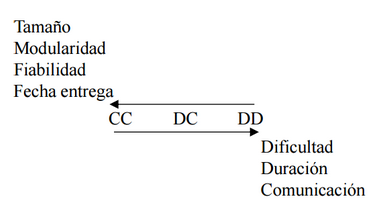
\includegraphics[width=0.6\textwidth]{images/dd.PNG}
	\caption{Tipos de estructura de equipos}
\end{figure}

La estructura de equipo \gls{dd} en la que nos basamos no tiene un líder de grupo permanente, aunque en nuestro caso, \textbf{David Cantador Piedras}, ha realizado el papel de gestor del proyecto, encargado de la organización (distribución del trabajo), motivación y de la resolución de problemas durante el desarrollo del proyecto. Por esa razón, se nombran coordinadores de tareas a corto plazo y se sustituyen por otros para diferentes tareas.

Las decisiones sobre problemas y los enfoques que va a tomar el proyecto, se hacen a consenso del grupo. La comunicación entre los miembros del equipo es horizontal (debido a la ausencia de un líder permanente), gracias a la cual la resolución de dudas o problemas se ve limitada a: compartir información y al apoyo entre los integrantes del grupo.

Por otro lado, conviene resaltar la importancia de la cohesión del grupo, la cual es imprescindible. Un equipo está ``cohesionado'' cuando todos sus miembros comparten un objetivo como enfoque común y luchan por conseguir los resultados deseados para el grupo por encima de los intereses individuales. Además, el respeto, la confianza y la tolerancia son básicas para alcanzar dicha cohesión necesaria, aceptando otros puntos de vista que nos permite enriquecernos y a facilitarnos la resolución de problemas que surjan. Por esa razón, para cada uno de los integrantes se requiere compromiso y esfuerzo, así como la existencia de un proyecto común.

\subsection{Informes de gestión}
Los proyectos de Software se componen de participantes que pueden clasificarse en una de las siguientes cinco categorías:

\begin{itemize}
	\item\textbf{Gestor superior y Gestor técnico del proyecto:}
	      \begin{itemize}
		      \item\textbf{David Cantador Piedras: }es el encargado de definir los aspectos del negocio que a menudo tienen una influencia significativa en el proyecto. Así como, la capacidad de resolver problemas, motivación, planificación y organización del proyecto. Entre sus competencias destacan: Experiencia en desarrollo de aplicaciones Java y C++ (Visual studio code), gestión de MySQL, uso de GIT (software de control de versiones) y conocimientos de IBM RSA (Rational Software Architect) y de Microsoft Proyect.
	      \end{itemize}
	\item\textbf{Profesionales:}
	      \begin{itemize}
		      \item\textbf{Alejandro Barrachina Argudo:} experiencia en desarrollo de aplicaciones Java y C++ (Visual studio code), gestión de MySQL, uso de GIT (software de control de versiones) y conocimientos de IBM RSA (Rational Software Architect) y de Microsoft Proyect.\\
		            Centrado en realizar un breve resumen a modo de introducción del proyecto (objetivos, propósitos…).
		      \item\textbf{Rodrigo Sosa Saéz:} experiencia en desarrollo de aplicaciones Java (Eclipse IDE for Java Developers) y C++, gestión de Oracle SQL Developer, Conocimientos de IBM RSA (Rational Software Architect), uso de GIT (software de control de versiones) y GitHub. \\
		            Centrado en la declaración de los recursos y personal necesarios para el desarrollo del proyecto.
		      \item\textbf{Juan Pantaleón Femenía Quevedo:} experiencia en desarrollo de aplicaciones Java (Eclipse IDE for Java Developers) y C++, uso de GIT (software de control de versiones) y GitHub, gestión de Oracle SQL Developer, Conocimientos de IBM RSA (Rational Software Architect) y Microsoft Proyect.\\
		            Su tarea se centra principalmente en la planificación temporal del trabajo.
		      \item\textbf{David Llanes Martín:} experiencia en desarrollo de aplicaciones Java (Eclipse IDE for Java Developers) y C++, gestión de Oracle SQL Developer, conocimientos de IBM RSA (Rational Software Architect), uso de GIT (software de control de versiones) y GitHub. \\
		            Su tarea está enfocada en la gestión de cambios y seguimiento en el proyecto.
		      \item\textbf{Sergio Sánchez Chamizo:} experiencia en desarrollo de aplicaciones Java (Eclipse IDE for Java Developers) y C++, gestión de Oracle SQL Developer, Conocimientos de IBM RSA (Rational Software Architect), uso de GIT (software de control de versiones) y GitHub y conocimientos de Microsoft Project.\\
		            Su labor está enfocada en la gestión de riesgos del proyecto.
		      \item\textbf{Samuel Rodrigo Moreno:} experiencia en desarrollo de aplicaciones Java (Eclipse IDE for Java Developers) y C++, conocimientos de Microsoft Project, gestión de Oracle SQL Developer, Conocimientos de IBM RSA (Rational Software Architect), uso de GIT (software de control de versiones) y GitHub.\\
		            Centrado en la estimación del proyecto con respecto a su coste, esfuerzo, etc.
		      \item\textbf{Rodrigo Souto Santos:} experiencia en desarrollo de aplicaciones Java (Eclipse IDE for Java Developers) y C++, conocimientos de Microsoft Project, uso de GIT (software de control de versiones), github, gestión de Oracle SQL Developer y conocimientos de IBM RSA (Rational Software Architect). \\
		            Su tarea está centrada en la gestión de los miembros que conforman el equipo de trabajo.
	      \end{itemize}
\end{itemize}

No obstante, todos los integrantes del grupo deberán colaborar en las diferentes partes del proyecto, con el objetivo de obtener un mejor resultado del mismo, además de la tarea explicita para cada uno de los miembros del equipo.

\begin{itemize}
	\item\textbf{Los clientes,} los cuales especifican los requisitos de la aplicación. Mantienen contacto con los profesionales al poderse modificar, añadir algún otro requisito al proyecto.
	\item\textbf{Los usuarios finales, }estarán formados por los trabajadores de las diferentes sucursales de la empresa y los clientes que empleen la aplicación de forma online o que acudan a los establecimientos, los cuales interactuarán con el software.
\end{itemize}

\newpage
\section{Mecanismos de seguimiento y control}
Para satisfacer el monitoreo del presente proyecto, se aplicarán series de inspecciones periódicas, de las cuales su tiempo de monitoreo dependerá de la evolución del software y la cantidad de fallos que este pueda producir en el tiempo. El encargado en realizar este seguimiento será un grupo especial o \gls{sqa}, el cual tendrá un jefe responsable de todos los cambios, soluciones y decisiones que se realicen en el mantenimiento, este jefe no es más que el mismo jefe del proyecto.

\subsection{Garantía de calidad y control (Plan de calidad)}
Para asegurar la calidad del producto (software), se realizarán verificaciones y revisiones técnicas formales.\\
El encargado de llevar a cabo todo esto será el jefe del grupo \gls{sqa}. Además, este grupo se encargará de ayudar a los desarrolladores para que el software alcance una calidad más alta.\\
El método que vamos a utilizar principalmente es el de realizar inspecciones. Su propósito es detectar e identificar anomalías en el producto software.\\
Esto nos servirá para:
\begin{itemize}
	\item  Verificar que el producto software satisface sus especificaciones.
	\item  Verificar que el producto software satisface los atributos de calidad especificados.
	\item Verificar que el producto software se ajuste a las regulaciones aplicables, estándares, guías, planes y procedimientos.
	\item  Identificar desviaciones con respecto a estándares y especificaciones.
	\item Recolectar datos de \gls{is}.
	\item utilizar los datos de \gls{is} recolectados para mejorar el proceso de inspección y su documentación de soporte.
\end{itemize}
Estos dos últimos puntos son opcionales, se puede llevar una eficiente gestión del proyecto con la ausencia de ellas, aun así, se recomienda utilizarlas para un control aún más óptimo del software.


Durante las inspecciones se determinarán las soluciones de las anomalías que se presenten. Esto servirá para revisar entre otras cosas: el diseño, el código fuente, y la documentación de usuarios.

Las inspecciones se llevarán a cabo de la siguiente manera:
\begin{enumerate}
	\item El responsable de llevar a cabo el producto informa del fin de un trabajo al jefe de proyecto.
	\item El jefe contacta con unos supervisores, a los cuales se les entrega el producto.
	\item Los supervisores se encargan de dar el visto bueno al proyecto durante horas.
	\item El jefe de trabajo planifica una reunión para una fecha lo más cercana posible.
	\item Uno de los supervisores actúa como testigo, este se encarga de anotar las incidencias.
	\item El creador del producto expone su producto.
	\item Los supervisores ponen pegas al producto.
	\item Cuando se descubre una incidencia el testigo las anota.
\end{enumerate}

Cuando acaba la reunión hay tres opciones: aceptar el producto sin modificaciones, rechazar el producto o aceptar el producto tras llevar a cabo unas modificaciones sin una nueva inspección.  Al finalizar la reunión, todos los participantes de la reunión firman el registro de revisión para de esta forma hacerlo oficial evitando riesgos legales o de contrato.


\subsection{Gestión y control de cambios (Plan GCS)}
Todos los miembros del proyecto podrán realizar una solicitud de cambio sobre alguno de los requerimientos del producto registrados. Para esto se deberá́ respetar el siguiente protocolo de trabajo:

\begin{itemize}
	\item Toda solicitud de cambio debe ser requerida con una justificación vía correo electrónico hacia el Jefe de Proyecto. Todo cambio realizado sin ser comunicado previamente por este medio no será aplicado a la línea base.
	\item Toda solicitud de cambio deberá ser analizada y aprobada por el Jefe de Proyecto con el soporte de la persona responsable del activo que se solicita modificar. Queda a su cargo la tarea de relevar cuál es el impacto que tendrá en el proyecto y realizar los ajustes pertinentes (reflejar en la documentación de cambios) para minimizar el mismo.
	\item Será el Jefe de Proyecto el encargado de informar al personal sobre la implementación de dicho cambio (en caso de que lo aprobara). Se utilizará la matriz que se encuentra en la sección “Plan de Gestión de la Configuración” para asignar al responsable de realizar el registro de cambio en la documentación de cambios.
	\item El jefe de proyecto evaluará las acciones correctivas y preventivas que se deberán aplicar.
	\item El líder de proyecto será responsable de verificar que se han realizado las modificaciones necesarias en los requerimientos del producto, que generaron la implementación del cambio aprobado.
	\item Luego que un cambio haya sido aprobado quedará a cargo del Líder del Proyecto la tarea de verificar que se ha registrado correctamente el cambio para mantener la integridad del proyecto.
\end{itemize}

\newpage
\printglossary[title=Apendice A. Glosario]
\newpage
\listof{table}{Apendice B. Cuadros}
\end{document}
